\section*{Глава 1\\Математические модели}
\addcontentsline{toc}{section}{Глава 1. Математические модели}
\setcounter{section}{1}
\setcounter{subsection}{0}

\subsection{Уравнения механики деформируемого твёрдого тела}
Для математического моделирования волновых процессов в деформируемом твёрдом
теле используется система динамических уравнений \cite{novatsky,sedov} в виде
\begin{align}
\label{initial_equations}
\rho\dot{v}_i &= \nabla_j\sigma_{ij}+f_i & \textrm{(уравнения движения)}\nonumber\\
\sigma_{ij} &= q_{ijkl}\dot{\varepsilon}_{kl}+F_{ij} & \textrm{(реологические
соотношения).}
\end{align}

Здесь $\rho$ – плотность среды, $v_i$ – компоненты скорости смещения,
$\sigma_{ij}$, $\varepsilon_{ij}$ -- компоненты тензоров напряжений и деформаций,
$\nabla_j$ – ковариантная производная по $j$-й координате, $f_i$ – массовые
силы, действующие на единицу объёма, $F_{ij}$ -- правая часть, используемая, например, для описания диссипации в моделях с учётом вязкости.

В случае малых деформаций тензор скоростей деформаций $e_{ij}=\dot{\varepsilon}_{ij}$ 
выражается через компоненты скорости смещения линейным образом \cite{landau_lifshits}:
\begin{equation}
e_{ij}=\frac{1}{2}(\nabla_j v_i+\nabla_i v_j).
\end{equation}

Вид компонент тензора 4-го порядка $q_{ijkl}$ и правой части $F_{ij}$ определяется реологией среды.

Для замыкания системы уравнений \ref{initial_equations} её необходимо дополнить
уравнением состояния, определяющим зависимость плотности от напряжений:
\begin{equation}
\rho=\rho_0e^{\frac{p}{K}},
\end{equation}
где $p=-\frac{1}{3}\sum\sigma_{kk}$ -- давление, $K=\lambda+\frac{2}{3}\mu$ --
коэффициент всестороннего сжатия, $\lambda$ и $\mu$ -- параметры Ламе.

Параметры Ламе зависят от материала и связаны с модулем продольной упругости и коэффициентом Пуассона следующим образом:
\begin{align}
\label{lame_parameters}
\lambda &= \frac{E\nu}{(1+\nu)(1-2\nu)}
\nonumber\\
\mu &= G=\frac{E}{2(1+\nu)}
\end{align}
Здесь $E$ -- модуль продольной упругости, $\nu$ -- коэффициент Пуассона, $G$ -- модуль сдвига.

В простейшем случае линейной упругости $q_{ijkl}=\lambda\delta_{ij}\delta_{kl}+\mu(\delta_{ik}\delta_{jl}+\delta_{il}\delta_{jk})$ и $F_{ij}=0$. Тогда в приближении малых деформаций и в отсутствии внешних сил в трехмерном пространстве и декартовых координатах уравнения \ref{initial_equations} принимают вид
\begin{align}
\label{simple_equations}
\frac{\partial{v_x}}{\partial{t}}&=\frac{1}{\rho}(\frac{\partial{\sigma_{xx}}}{\partial{x}}+\frac{\partial{\sigma_{xy}}}{\partial{y}}+\frac{\partial{\sigma_{xz}}}{\partial{z}})
\nonumber\\
\frac{\partial{v_y}}{\partial{t}}&=\frac{1}{\rho}(\frac{\partial{\sigma_{xy}}}{\partial{x}}+\frac{\partial{\sigma_{yy}}}{\partial{y}}+\frac{\partial{\sigma_{yz}}}{\partial{z}})
\nonumber\\
\frac{\partial{v_z}}{\partial{t}}&=\frac{1}{\rho}(\frac{\partial{\sigma_{xz}}}{\partial{x}}+\frac{\partial{\sigma_{yz}}}{\partial{y}}+\frac{\partial{\sigma_{zz}}}{\partial{z}})
\nonumber\\
\frac{\partial{\sigma_{xx}}}{\partial{t}}&=(\lambda+2\mu)\frac{\partial{v_x}}{\partial{x}}+\lambda\frac{\partial{v_y}}{\partial{y}}+\lambda\frac{\partial{v_z}}{\partial{z}}
\nonumber\\
\frac{\partial{\sigma_{xy}}}{\partial{t}}&=\mu(\frac{\partial{v_x}}{\partial{y}}+\frac{\partial{v_y}}{\partial{x}})
\nonumber\\
\frac{\partial{\sigma_{xz}}}{\partial{t}}&=\mu(\frac{\partial{v_x}}{\partial{z}}+\frac{\partial{v_z}}{\partial{x}})
\nonumber\\
\frac{\partial{\sigma_{yy}}}{\partial{t}}&=\lambda\frac{\partial{v_x}}{\partial{x}}+(\lambda+2\mu)\frac{\partial{v_y}}{\partial{y}}+\lambda\frac{\partial{v_z}}{\partial{z}}
\nonumber\\
\frac{\partial{\sigma_{yz}}}{\partial{t}}&=\mu(\frac{\partial{v_z}}{\partial{y}}+\frac{\partial{v_y}}{\partial{z}})
\nonumber\\
\frac{\partial{\sigma_{zz}}}{\partial{t}}&=\lambda\frac{\partial{v_x}}{\partial{x}}+\lambda\frac{\partial{v_y}}{\partial{y}}+(\lambda+2\mu)\frac{\partial{v_z}}{\partial{z}}
\end{align}

Очевидно, что уравнения \ref{simple_equations} можно переписать в матричной форме:
\begin{equation}
\label{simple_matrix_equation}
\frac{\partial\vec{u}}{\partial{t}}+\mathbf{A}_x\frac{\partial\vec{u}}{\partial{x}}+
\mathbf{A}_y\frac{\partial\vec{u}}{\partial{y}}+
\mathbf{A}_z\frac{\partial\vec{u}}{\partial{z}}=0.
\end{equation}
Здесь
$\vec{u}=\{v_x,v_y,v_z,\sigma_{xx},\sigma_{yy},\sigma_{zz},\sigma_{xy},\sigma_{xz},\sigma_{yz}\}^T$
-- вектор искомых функций, $x,y,z$ --  независимые пространственные переменные, $t$ -- время.

Аналогично можно записать более общую систему \ref{initial_equations} в виде:
\begin{equation}
\label{matrix_equation}
\frac{\partial\vec{u}}{\partial{t}}+\mathbf{A}_x\frac{\partial\vec{u}}{\partial{x}}+
\mathbf{A}_y\frac{\partial\vec{u}}{\partial{y}}+
\mathbf{A}_z\frac{\partial\vec{u}}{\partial{z}}=\vec{f}.
\end{equation}
Здесь $\vec{f}$ -- вектор правых частей, размерность которого равна размерности исходной системы, а выражения для компонентов зависят от реологии среды. Точный вид матриц $\mathbf{A}_x$, $\mathbf{A}_y$, $\mathbf{A}_z$ также зависит от реологии среды.

\clearpage
\newpage

\subsection{Приближение линейно упругого тела}
\label{elastic_matrixes}

Для линейно упругого тела тензор $q_{ijkl}$ и правая часть $F_{ij}$ в \ref{initial_equations} принимают следующий вид \cite{landau_lifshits}:
\begin{align}
\label{tensor_qijkl_elastic}
q_{ijkl}&=\lambda\delta_{ij}\delta_{kl}+\mu(\delta_{ik}\delta_{jl}+\delta_{il}
\delta_{jk}),\nonumber\\
F_{ij}&=0.
\end{align}
В этом соотношении $\lambda$ и $\mu$ -- параметры Ламе, $\delta_{ij}$ -- символ Кронекера.

Для линейно упругого тела матрицы $\mathbf{A}_x$, $\mathbf{A}_y$, $\mathbf{A}_z$ в \ref{matrix_equation} принимают следующий вид.

\begin{displaymath}
\mathbf{A}_x =
\left( \begin{array}{cccccccccccc}
0 & 0 & 0 & -\frac 1 \rho & 0 & 0 & 0 & 0 & 0 \\ 
0 & 0 & 0 & 0 & -\frac 1 \rho & 0 & 0 & 0 & 0 \\ 
0 & 0 & 0 & 0 & 0 & -\frac 1 \rho & 0 & 0 & 0 \\ 
-(\lambda+2\mu) & 0 & 0 & 0 & 0 & 0 & 0 & 0 & 0 \\ 
0 & -\mu & 0 & 0 & 0 & 0 & 0 & 0 & 0 \\ 
0 & 0 & -\mu & 0 & 0 & 0 & 0 & 0 & 0 \\ 
-\lambda & 0 & 0 & 0 & 0 & 0 & 0 & 0 & 0 \\ 
0 & 0 & 0 & 0 & 0 & 0 & 0 & 0 & 0 \\ 
-\lambda & 0 & 0 & 0 & 0 & 0 & 0 & 0 & 0  
\end{array} \right),
\end{displaymath} 
\begin{displaymath}
\mathbf{A}_y =
\left( \begin{array}{cccccccccccc}
0 & 0 & 0 & 0 & -\frac 1 \rho & 0 & 0 & 0 & 0 \\ 
0 & 0 & 0 & 0 & 0 & 0 & -\frac 1 \rho & 0 & 0 \\ 
0 & 0 & 0 & 0 & 0 & 0 & 0 & -\frac 1 \rho & 0 \\ 
0 & -\lambda & 0 & 0 & 0 & 0 & 0 & 0 & 0 \\ 
-\mu & 0 & 0 & 0 & 0 & 0 & 0 & 0 & 0 \\ 
0 & 0 & 0 & 0 & 0 & 0 & 0 & 0 & 0 \\ 
0 & -(\lambda+2\mu) & 0 & 0 & 0 & 0 & 0 & 0 & 0 \\ 
0 & 0 & -\mu & 0 & 0 & 0 & 0 & 0 & 0 \\ 
0 & -\lambda & 0 & 0 & 0 & 0 & 0 & 0 & 0  
\end{array} \right),
\end{displaymath}
\begin{displaymath}
\mathbf{A}_z =
\left( \begin{array}{cccccccccccc}
0 & 0 & 0 & 0 & 0 & -\frac 1 \rho & 0 & 0 & 0 \\ 
0 & 0 & 0 & 0 & 0 & 0 & 0 & -\frac 1 \rho & 0 \\ 
0 & 0 & 0 & 0 & 0 & 0 & 0 & 0 & -\frac 1 \rho \\ 
0 & 0 & -\lambda & 0 & 0 & 0 & 0 & 0 & 0 \\ 
0 & 0 & 0 & 0 & 0 & 0 & 0 & 0 & 0 \\ 
-\mu & 0 & 0 & 0 & 0 & 0 & 0 & 0 & 0 \\ 
0 & 0 & -\lambda & 0 & 0 & 0 & 0 & 0 & 0 \\ 
0 & -\mu & 0 & 0 & 0 & 0 & 0 & 0 & 0 \\ 
0 & 0 & -(\lambda+2\mu) & 0 & 0 & 0 & 0 & 0 & 0  
\end{array} \right).
\end{displaymath}

%\todo{Добавить полное исследование системы и явный вид матриц $\Lambda$ и $\Omega$.}

\clearpage
\newpage

\subsection{Приближение упруго-пластического тела}

\subsubsection{Модель Прандтля-Рейсса}
\label{plastic_matrixes}

Для упруго-пластического тела используется модель Прандтля-Рейсса с условием текучести Мизеса. Тогда тензор $q_{ijkl}$ и правая часть $F_{ij}$ в \ref{initial_equations} имеют более сложный вид \cite{ivanov_kondaurov_petrov_holodov, g}:
\begin{align}
\label{tensor_qijkl_plastic}
q_{ijkl}&=\lambda\delta_{ij}\delta_{kl}+\mu(\delta_{ik}\delta_{jl}+\delta_{il}\delta_{jk})-\frac{I\mu\sigma_{ij}\sigma_{kl}}{K^2},
\nonumber\\
F_{ij}&=0.
\end{align}
В этом соотношении $\lambda$ и $\mu$ -- параметры Ламе, $K$ -- предел текучести на сдвиг, $\sigma_{ij}$ -- компоненты тензора напряжений, $\delta_{ij}$ -- символ Кронекера, $I$ -- параметр модели, который определяется следующим образом:

\begin{equation}
\label{I_parameter_plastic}
I=\begin{cases}
0, & \text{если $S = \sigma_{xx}^2+\sigma_{yy}^2+\sigma_{zz}^2+2\sigma_{xy}^2+2\sigma_{xz}^2+2\sigma_{yz}^2 < 2K^2$}\\
1, & \text{если $S \ge 2K^2$}.
\end{cases}
\end{equation}

Для линейно упругого тела матрицы $\mathbf{A}_x$, $\mathbf{A}_y$, $\mathbf{A}_z$ в \ref{matrix_equation} имеют существенно более сложный вид, так как компоненты тензора $q_{ijkl}$ зависят от компонентов тензора $\sigma$. Значения $\sigma_{ij}$ в общем случае различны в каждой точке пространства в каждый момент времени. Это приводит к тому, что невозможно упростить вид матриц аналитически и получить их покомпонентную запись в терминах $\lambda, \mu, \rho$, как это было сделано для линейно упругого тела. Значения ненулевых элементов каждой матрицы необходимо вычислять в каждой точке пространства в каждый момент времени в соответствии с \ref{tensor_qijkl_plastic} и \ref{I_parameter_plastic}, используя текущие значения $\sigma_{ij}$ в данной точке.

\begin{displaymath}
\mathbf{A}_x =
\left( \begin{array}{cccccccccccc}
0 & 0 & 0 & -\frac 1 \rho & 0 & 0 & 0 & 0 & 0 \\ 
0 & 0 & 0 & 0 & -\frac 1 \rho & 0 & 0 & 0 & 0 \\ 
0 & 0 & 0 & 0 & 0 & -\frac 1 \rho & 0 & 0 & 0 \\ 
-q_{1111} & -\frac{q_{1112}+q_{1121}}{2} & -\frac{q_{1113}+q_{1131}}{2} & 0 & 0 & 0 & 0 & 0 & 0 \\ 
-q_{1211} & -\frac{q_{1212}+q_{1221}}{2} & -\frac{q_{1213}+q_{1231}}{2} & 0 & 0 & 0 & 0 & 0 & 0 \\ 
-q_{1311} & -\frac{q_{1312}+q_{1321}}{2} & -\frac{q_{1313}+q_{1331}}{2} & 0 & 0 & 0 & 0 & 0 & 0 \\ 
-q_{2211} & -\frac{q_{2212}+q_{2221}}{2} & -\frac{q_{2213}+q_{2231}}{2} & 0 & 0 & 0 & 0 & 0 & 0 \\ 
-q_{2311} & -\frac{q_{2312}+q_{2321}}{2} & -\frac{q_{2313}+q_{2331}}{2} & 0 & 0 & 0 & 0 & 0 & 0 \\ 
-q_{3311} & -\frac{q_{3312}+q_{3321}}{2} & -\frac{q_{3313}+q_{3331}}{2} & 0 & 0 & 0 & 0 & 0 & 0  
\end{array} \right),
\end{displaymath} 
\begin{displaymath}
\mathbf{A}_y =
\left( \begin{array}{cccccccccccc}
0 & 0 & 0 & 0 & -\frac 1 \rho & 0 & 0 & 0 & 0 \\ 
0 & 0 & 0 & 0 & 0 & 0 & -\frac 1 \rho & 0 & 0 \\ 
0 & 0 & 0 & 0 & 0 & 0 & 0 & -\frac 1 \rho & 0 \\ 
-\frac{q_{1112}+q_{1121}}{2} & -q_{1122} & -\frac{q_{1123}+q_{1132}}{2} & 0 & 0 & 0 & 0 & 0 & 0 \\ 
-\frac{q_{1212}+q_{1221}}{2} & -q_{1222} & -\frac{q_{1223}+q_{1232}}{2} & 0 & 0 & 0 & 0 & 0 & 0 \\ 
-\frac{q_{1312}+q_{1321}}{2} & -q_{1322} & -\frac{q_{1323}+q_{1332}}{2} & 0 & 0 & 0 & 0 & 0 & 0 \\ 
-\frac{q_{2212}+q_{2221}}{2} & -q_{2222} & -\frac{q_{2223}+q_{2232}}{2} & 0 & 0 & 0 & 0 & 0 & 0 \\ 
-\frac{q_{2312}+q_{2321}}{2} & -q_{2322} & -\frac{q_{2323}+q_{2332}}{2} & 0 & 0 & 0 & 0 & 0 & 0 \\ 
-\frac{q_{3312}+q_{3321}}{2} & -q_{3322} & -\frac{q_{3323}+q_{3332}}{2} & 0 & 0 & 0 & 0 & 0 & 0  
\end{array} \right),
\end{displaymath}
\begin{displaymath}
\mathbf{A}_z =
\left( \begin{array}{cccccccccccc}
0 & 0 & 0 & 0 & 0 & -\frac 1 \rho & 0 & 0 & 0 \\ 
0 & 0 & 0 & 0 & 0 & 0 & 0 & -\frac 1 \rho & 0 \\ 
0 & 0 & 0 & 0 & 0 & 0 & 0 & 0 & -\frac 1 \rho \\ 
-\frac{q_{1113}+q_{1131}}{2} & -\frac{q_{1123}+q_{1132}}{2} & -q_{1133} & 0 & 0 & 0 & 0 & 0 & 0 \\ 
-\frac{q_{1213}+q_{1231}}{2} & -\frac{q_{1223}+q_{1232}}{2} & -q_{1233} & 0 & 0 & 0 & 0 & 0 & 0 \\ 
-\frac{q_{1313}+q_{1331}}{2} & -\frac{q_{1323}+q_{1332}}{2} & -q_{1333} & 0 & 0 & 0 & 0 & 0 & 0 \\ 
-\frac{q_{2213}+q_{2231}}{2} & -\frac{q_{2223}+q_{2232}}{2} & -q_{2233} & 0 & 0 & 0 & 0 & 0 & 0 \\ 
-\frac{q_{2313}+q_{2331}}{2} & -\frac{q_{2323}+q_{2332}}{2} & -q_{2333} & 0 & 0 & 0 & 0 & 0 & 0 \\ 
-\frac{q_{3313}+q_{3331}}{2} & -\frac{q_{3323}+q_{3332}}{2} & -q_{3333} & 0 & 0 & 0 & 0 & 0 & 0  
\end{array} \right).
\end{displaymath}

%\todo{Добавить про вид матриц $\Lambda$ и $\Omega$.}

\clearpage
\newpage

\subsection{Приближение вязко-упругого тела}

\subsubsection{Модель Максвелла}
\label{viscosity_matrixes}

Для вязко-упругого тела при использовании модели Максвелла тензор $q_{ijkl}$ и правая часть $F_{ij}$ в \ref{initial_equations} принимают следующий вид \cite{godunov_phys}:
\begin{align}
\label{tensor_qijkl_viscosity}
q_{ijkl}&=\lambda\delta_{ij}\delta_{kl}+\mu(\delta_{ik}\delta_{jl}+\delta_{il}
\delta_{jk}),\nonumber\\
F_{ij}&=-\frac{\sigma_{ij}}{\tau_0}.
\end{align}
В этом соотношении $\lambda$ и $\mu$ -- параметры Ламе, $\delta_{ij}$ -- символ Кронекера, $\tau_0$ -- время релаксации.


Для вязко-упругого тела матрицы $\mathbf{A}_x$, $\mathbf{A}_y$, $\mathbf{A}_z$ в \ref{matrix_equation} принимают вид, полностью совпадающий со случаем линейно упругого тела (см.раздел\ref{elastic_matrixes}). Отличия только в правой части уравнений, в которой для вязко-упругого тела возникают члены, отвечающие за диссипацию.


\subsubsection{Модель Работнова}
\label{rabotnov_matrixes}

При использовании модели Работнова наследственной вязко-упругой среды тензор $q_{ijkl}$ и правая часть $F_{ij}$ в \ref{initial_equations} принимают следующий вид \cite{rabotnov, polilov}:
\begin{align}
\label{tensor_qijkl_rabotnov}
q_{ijkl}&=\lambda\delta_{ij}\delta_{kl}+\mu(\delta_{ik}\delta_{jl}+\delta_{il}
\delta_{jk}),\nonumber\\
F_{ij}&=-(L^*+M^*)\sigma_{ij}.
\end{align}
В этом соотношении $\lambda$ и $\mu$ -- параметры Ламе, $\delta_{ij}$ -- символ Кронекера. Правая часть имеет достаточно сложный вид и описывает поведение материала с учетом истории его нагружения. Оператор $L^*$ учитывает вязкие эффекты, оператор $M^*$ -- накопление повреждений. Вид операторов:
\begin{align}
\label{right_hand_rabotnov}
L^*\sigma_{ij} &= \int_0^T{K_L(1-\tau)\sigma_{ij}d\tau}, \nonumber\\
M^*\sigma_{ij} &= \int_0^T{K_M(1-\tau)\sigma_{ij}d\tau}, \nonumber\\
K_L(1-\tau)&=\rho(1-\tau)^{-\alpha}, \nonumber\\
K_M(1-\tau)&=m(1-\tau)^{-\alpha}.
\end{align}
Здесь $K_L(1-\tau)$ и $K_M(1-\tau)$ -- разностные ядра Абеля.

При использовании модели Работнова уравнения перестают быть локальными, для поиска решения на временном слое $n+1$ требуется интегрирование, вообще говоря, за все время жизни среды.

Для модели Работнова матрицы $\mathbf{A}_x$, $\mathbf{A}_y$, $\mathbf{A}_z$ в \ref{matrix_equation} принимают вид, полностью совпадающий со случаем линейно упругого тела (см.раздел\ref{elastic_matrixes}). Отличия только в правой части уравнений, в которой возникают члены, отвечающие за вязкие эффекты и накопление повреждений.

\clearpage
\newpage

\subsection{Приближение вязко-упруго-пластического тела}

\subsubsection{Модель Кукуджанова}
\label{kukudzhanov_matrixes}

Для вязко-упруго-пластического тела при использовании модели Кукуджанова тензор $q_{ijkl}$ и правая часть $F_{ij}$ в \ref{initial_equations} принимают следующий вид \cite{kukudzhanov, p21, p27}:
\begin{align}
\label{tensor_qijkl_kukudzhanov}
q_{ijkl}&=\lambda\delta_{ij}\delta_{kl}+\mu(\delta_{ik}\delta_{jl}+\delta_{il}
\delta_{jk}),\nonumber\\
F_{ij}&=-\frac{2\mu}{\tau_0\sigma_{kl}\sigma_{kl}} F(\sigma_{kl},\sigma_{kl},K)\sigma_{ij},\nonumber\\
F(\sigma_{kl},\sigma_{kl},K) &= \frac{(\sigma_{kl},\sigma_{kl})^{1/2}-(2K)^{1/2}}{\tau_0(\sigma_{kl},\sigma_{kl})^{1/2}}
\end{align}
В этом соотношении $\lambda$ и $\mu$ -- параметры Ламе, $\delta_{ij}$ -- символ Кронекера, $\tau_0$ -- время релаксации, $K$ -- предел текучести на сдвиг.

Для вязко-упруго-пластического тела матрицы $\mathbf{A}_x$, $\mathbf{A}_y$, $\mathbf{A}_z$ в \ref{matrix_equation} принимают вид, полностью совпадающий со случаем линейно упругого тела (см.раздел\ref{elastic_matrixes}). Отличия только в правой части уравнений.


\clearpage
\newpage

\subsection{Моделирование композиционных материалов}

Композиционными называют материалы, состоящие из двух или более компонентов или фаз и удовлетворяющие следующим условиям:
\begin{itemize}
\item доля каждого компонента составляет не менее 5\% по объему;
\item свойства компонентов существенно различаются, как следствие свойства композита отличаются от свойств исходных компонентов;
\item композит получен путем смешения исходных компонентов.
\end{itemize}

В зависимости от того, как именно компоненты формируют итоговый материал, композиты могут иметь принципиально разную структуру \cite{bazhenov}. На рис. \ref{pic:composite-types} схематично показаны некоторые типы композитов.

\begin{figure}[h]
\centering
\begin{subfigure}[b]{0.2\textwidth}
\centering
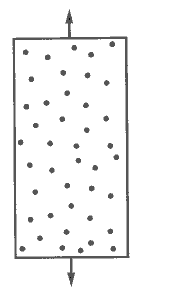
\includegraphics[width=\textwidth]{png/composites-types-1.png}
\caption{ }
\end{subfigure}
\begin{subfigure}[b]{0.2\textwidth}
\centering
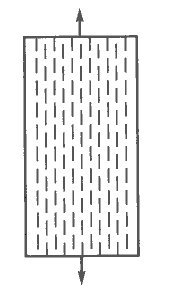
\includegraphics[width=\textwidth]{png/composites-types-2.png}
\caption{ }
\end{subfigure}
\begin{subfigure}[b]{0.2\textwidth}
\centering
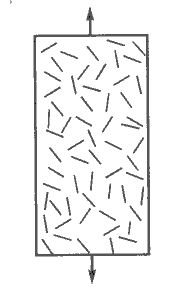
\includegraphics[width=\textwidth]{png/composites-types-3.png}
\caption{ }
\end{subfigure}
\begin{subfigure}[b]{0.2\textwidth}
\centering
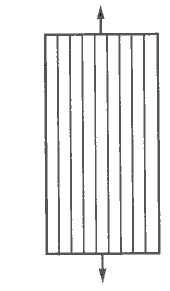
\includegraphics[width=\textwidth]{png/composites-types-4.png}
\caption{ }
\end{subfigure}
\caption{Типы композитов. а -- наполненный случайно распределенными частицами. б -- однонаправленные короткие волокна. в -- случайно ориентированные короткие волокна. г -- однонаправленные длинные волокна.}
\label{pic:composite-types}
\end{figure}

Свойства композитов определяются двумя факторами -- свойствами исходных компонентов и структурой их упаковки в итоговый композиционный материал. Для большинства композитов характерно наличие нескольких уровней структуры. Обычно можно выделить макроструктуру, микроструктуру и наноструктуру.

К макроструктуре относятся элементы структуры, размер которых сопоставим с размером итогового изделия. Например, в плетеной композитной ткани макроструктура включает в себя форму тканевых полос и метод плетения. К микроструктуре относятся элементы размером от единиц до сотен микрон. Этот уровень включает в себя волокна и матрицу, частицы наполнителя, поры, трещины и т.д. Наноструктура оперирует отдельными атомами и молекулами.

Принципиальные свойства композитов, отличающие их от других классов материалов, формируются как правило на микроуровне. На этом уровне композит состоит из двух (или более) компонентов. Непрерывная фаза называется матрицей, второй компонент -- наполнителем или армирующей фазой.

Матрица может быть керамической, металлической или полимерной. Очевидно, что механические свойства композитов с матрицами разных классов значительно отличаются. Полимеры являются самыми легкими из всех типов, но при этом менее жесткие и прочные. Керамические матрицы прочные, жесткие и хрупкие. Металлы занимают среднее положение по прочности и жесткости, при этом они пластичны.

Наполнитель как правило прочнее и жестче матрицы. Исключения встречаются, но они довольно редки. Форма наполнителя и его упаковка в значительной степени определяют механические свойства итогового композита. Различают два основные типа наполнителей -- волокнистые и дисперсные (см. рис. \ref{pic:composite-types}).

Механические свойства композита (жесткость, прочность) зависят от многих факторов \cite{rosen, guz}. Основными, безусловно, являются свойства матрицы и наполнителя и доля наполнителя в матрице. Для волокнистых композитов также важны форма, размер и ориентация волокон. Для прочности композита, помимо прочности компонентов, также принципиальна адгезионная прочность между матрицей и волокнами. Причем на свойствах композита плохо сказывается как слишком низкая, так и слишком высокая адгезия. Если адгезионная прочность низкая, то нагрузка не передается от матрицы к волокнам, что приводит к быстрому разрушению матрицы. Но если адгезия слишком высока, волокна совсем не отслаиваются от матрицы, и композит становится хрупким \cite{regel, deteresa}.

Таким образом, при рассмотрении свойств композита приходится учитывать множество факторов и параметров. Для определения эффективных характеристик композиционных материалов в настоящее время как правило применяются многомасштабные методы, разработанные под руководством Н.С. Бахвалова \cite{bahvalov}. Многомасштабные методы позволяют осреднить упругие характеристики материала и заменить его эквивалентной однородной средой с эффективными характеристиками \cite{dimitrienko1, dimitrienko2}.

В данной работе для моделирования разрушения композиционных материалов применяется сочетание использования осредненных характеристик и прямого численного моделирования без осреднения. Так при моделировании обшивки самолета, состоящей из нескольких композитных субпакетов, каждый отдельный субпакет заменяется однородной средой с эффективными характеристиками, но при этом границы между отдельными субпакетами выделяются явно, что позволяет учесть отражение и преломление упругих волн на контактных границах.


\clearpage
\newpage

\subsection{Преобразование уравнений при смене базиса}

При практической реализации численного метода для решения системы \ref{matrix_equation} достаточно часто возникает необходимость смены базиса. Это может быть связано, например, с необходимостью случайного выбора направления координатных осей. Случайный выбор базиса используется для того, чтобы исключить наличие выделенных направлений, которые приводят к анизотропии численного решения. Еще одной частой причиной смены базиса является расчет областей с границей сложной формы. В этом случае при расчете граничных точек метод может требовать определенной ориентации осей базиса относительно внешней нормали в данной точке границы.

Исследуем, как преобразуются уравнения при смене базиса. Для этого рассмотрим исходный базис $\vec x = (x, y, z)^T$ и новый базис $\vec \xi = (\xi, \eta, \zeta)^T$. Пусть $\mathbf G$ - матрица, столбцами которой являются координаты векторов нового базиса $\vec \xi$ в старом базисе $\vec x$.

Тогда координаты точек, их скорости, а также компоненты тензора напряжений при переходе между базисами преобразуются следующим образом:
\begin{align}
\label{basis_change}
\vec r_x &= \mathbf G \vec r_{\xi},
\nonumber\\
\vec v_x &= \mathbf G \vec v_{\xi},
\nonumber\\
\vec \sigma_x &= \mathbf G \sigma_{\xi} \mathbf G,
\nonumber\\
\vec r_{\xi} &= {\mathbf G}^{-1} \vec r_x,
\nonumber\\
\vec v_{\xi} &= {\mathbf G}^{-1} \vec v_x,
\nonumber\\
\vec \sigma_{\xi} &= {\mathbf G}^{-1} \sigma_x {\mathbf G}^{-1}.
\end{align}

Здесь индекс $x$ относится к величинам, заданным в старом базисе, а индекс $\xi$ -- в новом.

При программной реализации того или иного метода решения системы \ref{matrix_equation} удобно задавать входные параметры и получать результаты в некоторой фиксированной декартовой системе координат $\vec x$, так как такой формат является естественным для предметной области. Что принципиально с точки зрения реализации метода -- уравнения \ref{matrix_equation} записаны в форме, независимой от выбора той или иной системы координат. Поэтому можно хранить состояние среды (компоненты скорости и напряжения) в фиксированном базисе $\vec x$, а вычисления вести в некотором локальном базисе $\vec \xi$, удобном с точки зрения алгоритма численного метода и локальной конфигурации узлов расчётной сетки. В этом случае необходимо лишь специально указать, какие операторы подставлять вместо компонент градиента.

Переход к производным по направлениям нового базиса в \ref{matrix_equation} приводит к следующим преобразованиям:
\begin{align}
\nonumber
\vec{f} &= \frac{\partial\vec{u}}{\partial{t}} + 
\mathbf{A}_x\frac{\partial\vec{u}}{\partial{x}} + 
\mathbf{A}_y\frac{\partial\vec{u}}{\partial{y}} + 
\mathbf{A}_z\frac{\partial\vec{u}}{\partial{z}} =
& \nonumber\\
&= \frac{\partial\vec{u}}{\partial{t}} + 
\mathbf{A}_x (\frac{\partial\vec{u}}{\partial{\xi}}\frac{\partial{\xi}}{\partial{x}} + 
\frac{\partial\vec{u}}{\partial{\eta}}\frac{\partial{\eta}}{\partial{x}} + 
\frac{\partial\vec{u}}{\partial{\zeta}}\frac{\partial{\zeta}}{\partial{x}} ) + 
& \nonumber\\
& + \mathbf{A}_y (\frac{\partial\vec{u}}{\partial{\xi}}\frac{\partial{\xi}}{\partial{y}} + 
\frac{\partial\vec{u}}{\partial{\eta}}\frac{\partial{\eta}}{\partial{y}} + 
\frac{\partial\vec{u}}{\partial{\zeta}}\frac{\partial{\zeta}}{\partial{y}} ) + 
& \nonumber\\
& + \mathbf{A}_z (\frac{\partial\vec{u}}{\partial{\xi}}\frac{\partial{\xi}}{\partial{z}} + 
\frac{\partial\vec{u}}{\partial{\eta}}\frac{\partial{\eta}}{\partial{z}} + 
\frac{\partial\vec{u}}{\partial{\zeta}}\frac{\partial{\zeta}}{\partial{z}} ) = 
& \nonumber\\
& = \frac{\partial\vec{u}}{\partial{t}} + 
( \frac{\partial{\xi}}{\partial{x}} \mathbf{A}_x  + 
\frac{\partial{\xi}}{\partial{y}} \mathbf{A}_y + 
\frac{\partial{\xi}}{\partial{z}} \mathbf{A}_z ) \frac{\partial\vec{u}}{\partial{\xi}} + 
& \nonumber\\
& + ( \frac{\partial{\eta}}{\partial{x}} \mathbf{A}_x + 
\frac{\partial{\eta}}{\partial{y}} \mathbf{A}_y + 
\frac{\partial{\eta}}{\partial{z}} \mathbf{A}_z ) \frac{\partial\vec{u}}{\partial{\eta}} + 
& \nonumber\\
& + ( \frac{\partial{\zeta}}{\partial{x}} \mathbf{A}_x  + 
\frac{\partial{\zeta}}{\partial{y}} \mathbf{A}_y + 
\frac{\partial{\zeta}}{\partial{z}} \mathbf{A}_z ) \frac{\partial\vec{u}}{\partial{\zeta}}.
\end{align}

Таким образом, уравнение \ref{matrix_equation} после замены базиса имеет вид:
\begin{align}
\label{matrix_equation_generalized}
\frac{\partial\vec{u}}{\partial{t}} + 
( \xi_x \mathbf{A}_x  + \xi_y \mathbf{A}_y + \xi_z \mathbf{A}_z ) \frac{\partial\vec{u}}{\partial{\xi}} + 
( \eta_x \mathbf{A}_x + \eta_y \mathbf{A}_y + \eta_z \mathbf{A}_z ) \frac{\partial\vec{u}}{\partial{\eta}} + \nonumber\\
+ ( \zeta_x \mathbf{A}_x  + \zeta_y \mathbf{A}_y + \zeta_z \mathbf{A}_z ) \frac{\partial\vec{u}}{\partial{\zeta}} = \vec f.
\end{align}

Или, после замены обозначений:
\begin{equation}
\label{matrix_equation_generalized_short}
\frac{\partial\vec{u}}{\partial{t}} + \mathbf{A}_\xi \frac{\partial\vec{u}}{\partial{\xi}} + 
\mathbf{A}_\eta \frac{\partial\vec{u}}{\partial{\eta}} + \mathbf{A}_\zeta \frac{\partial\vec{u}}{\partial{\zeta}} = \vec f.
\end{equation}

Из вида уравнений \ref{matrix_equation_generalized} и \ref{matrix_equation_generalized_short} очевидным образом возникает задача исследования матрицы общего вида:
\begin{equation}
\label{matrix_generalized}
\mathbf{A}_q = q_x \mathbf{A}_x  + q_y \mathbf{A}_y + q_z \mathbf{A}_z,
\end{equation}
где $\mathbf{A}_q$ -- обобщенный вид матрицы, возникающей при переходе в новую систему координат, $q_x$ -- производные базисных векторов нового базиса по старому базису. В случае, когда оба базиса ортонормированные,
\begin{equation}
\label{good_basis_condition}
q_x^2 + q_y^2 + q_z^2 = 1.
\end{equation}
Уравнения \ref{matrix_equation_generalized}, \ref{matrix_equation_generalized_short} и \ref{matrix_generalized} верны и в случае произвольных базисов, в том числе неортогональных, но соотношение \ref{good_basis_condition} в этом случае уже не выполняется.

\subsubsection{Исследование матрицы общего вида $\mathbf{A}_q$}

Рассмотрим частный, но важный случай линейно упругого тела. Он представляет отдельный интерес, так как позволяет получить все необходимые соотношения в аналитическом виде явным образом, и таким образом исследовать, как отражается смена базиса на полной схеме построения численного метода. Кроме того, для большинства рассмотренных моделей вид матриц $\mathbf A_{x_i}$ совпадает с их видом для линейно упругого тела.

В случае линейной упругости в обобщенную матрицу \ref{matrix_generalized} входят матрицы $\mathbf{A}_x, \mathbf{A}_y, \mathbf{A}_z$, явный вид которых приведен в разделе \ref{elastic_matrixes}. Получаем следующий вид обобщенной матрицы $A_q$ (с точностью до знака):

\begin{equation}
\label{matrix_generalized_elastic}
\left( \begin{array}{cccccccccccc}
0 & 0 & 0 & \frac 1 \rho q_x & \frac 1 \rho q_y & \frac 1 \rho q_z & 0 & 0 & 0 \\ 
0 & 0 & 0 & 0 & \frac 1 \rho q_x & 0 & \frac 1 \rho q_y & \frac 1 \rho q_z & 0 \\ 
0 & 0 & 0 & 0 & 0 & \frac 1 \rho q_x & 0 & \frac 1 \rho q_y & \frac 1 \rho q_z \\ 
(\lambda+2\mu) q_x & \lambda q_y & \lambda q_z & 0 & 0 & 0 & 0 & 0 & 0 \\ 
\mu q_y & \mu q_x & 0 & 0 & 0 & 0 & 0 & 0 & 0 \\ 
\mu q_z & 0 & \mu q_x & 0 & 0 & 0 & 0 & 0 & 0 \\ 
\lambda q_x & (\lambda+2\mu) q_y & \lambda q_z & 0 & 0 & 0 & 0 & 0 & 0 \\ 
0 & \mu q_z & \mu q_y & 0 & 0 & 0 & 0 & 0 & 0 \\ 
\lambda q_x & \lambda q_y & (\lambda+2\mu) q_z & 0 & 0 & 0 & 0 & 0 & 0  
\end{array} \right)
\end{equation}

Полученная матрица имеет следующую структуру:

\begin{align}
- \mathbf{A}_q &=
\left( \begin{array}{cccccccccccc}
0 & \mathbf{B} \\
\mathbf{C} & 0
\end{array} \right),
\nonumber\\
\mathbf{B} &= 
\left( \begin{array}{cccccccccccc}
\frac 1 \rho q_x & \frac 1 \rho q_y & \frac 1 \rho q_z & 0 & 0 & 0 \\ 
0 & \frac 1 \rho q_x & 0 & \frac 1 \rho q_y & \frac 1 \rho q_z & 0 \\ 
0 & 0 & \frac 1 \rho q_x & 0 & \frac 1 \rho q_y & \frac 1 \rho q_z 
\end{array} \right),
\nonumber\\
\mathbf{C} &= 
\left( \begin{array}{cccccccccccc}
(\lambda+2\mu) q_x & \lambda q_y & \lambda q_z \\ 
\mu q_y & \mu q_x & 0 \\ 
\mu q_z & 0 & \mu q_x \\ 
\lambda q_x & (\lambda+2\mu) q_y & \lambda q_z \\ 
0 & \mu q_z & \mu q_y \\ 
\lambda q_x & \lambda q_y & (\lambda+2\mu) q_z  
\end{array} \right)
\end{align}

При нахождении собственных значений и векторов по методу Челнокова \cite{chelnokov} задача сводится к нахождению их для матрицы $\mathbf{C}^T \mathbf{B}^T$, которая имеет следующий вид:

\begin{align}
\frac 1 \rho 
\left( \begin{array}{cccccccccccc}
(\lambda+2\mu) q_x^2 + \mu q_y^2 + \mu q_z^2 & (\lambda+\mu) q_x q_y & (\lambda+\mu) q_x q_z \\
(\lambda+\mu) q_x q_y & \mu q_x^2 + (\lambda+2\mu) q_y^2 + \mu q_z^2 & (\lambda+\mu) q_y q_z \\
(\lambda+\mu) q_x q_z & (\lambda+\mu) q_y q_z & \mu q_x^2 + \mu q_y^2 + (\lambda+2\mu) q_z^2  
\end{array} \right).
\end{align} 

Собственные числа имеют вид:
\begin{align}
\left( \begin{array}{cccccccccccc}
\lambda_1 \\
\lambda_2 \\
\lambda_3 
\end{array} \right) = 
\frac 1 \rho (q_x^2 + q_y^2 + q_z^2)
\left( \begin{array}{cccccccccccc}
(\lambda+2\mu) \\
\mu \\
\mu  
\end{array} \right).
\end{align} 

Таким образом, при смене базиса собственные числа $\lambda_i$ меняются в $q_x^2 + q_y^2 + q_z^2$ раз. Если оба базиса ортонормированные, то соотношение \ref{good_basis_condition} выполняется и собственные числа не меняются при смене базиса. В случае же перехода в неортонормированный базис собственные числа могут меняться в широком диапазоне.

От $\lambda_i$ напрямую зависит, какие точки на предыдущем шаге по времени будут нужны для реконструкции решения на новом временном слое. Чем больше значения $\lambda_i$, тем больше угол наклона характеристики (см. разделы \ref{sec:hyperbolic_features} и \ref{sec:gcm_method_idea}). При увеличении $\lambda_i$ следует ожидать уменьшения допустимого шага по времени (при использовании курантовского ограничения на шаг $\lambda\tau / h \le 1$), либо (при попытке сохранить шаг по времени неизменным) еще более неприятных последствий, таких как появление непредусмотренных характеристик, выводящих за пределы расчетной области. Действительно, экспериментально было получено, что при попытке использовать неортогональный базис для расчета граничных узлов происходит увеличение $\lambda_i$ при переходе в новый базис и проявляются оба эти эффекта.

\clearpage
\newpage

\subsection{Свойства тензора напряжений}

\subsubsection{Нормальные и касательные напряжения}

Вектор напряжения $\mathbf{T}$, действующий на произвольную площадку, заданную нормалью $\mathbf n$, имеет вид
\begin{align}
\mathbf{T}^{(\mathbf n)}= \boldsymbol{\sigma}\cdot\mathbf n.
\end{align}

Нормальная часть напряжения очевидно равняется скалярному произведению вектора напряжения и нормали к площадке. Выражая через компоненты тензора напряжений и компоненты вектора нормали получаем
\begin{align}
\sigma_\mathrm{n} = \mathbf{T}^{(\mathbf{n})}\cdot \mathbf{n} = T^{(\mathbf n)}_i n_i = \sigma_{ij}n_i n_j.
\end{align}

Величина касательного напряжения к данной площадке выражается через полный вектор напряжения и нормальную составляющую напряжения
\begin{align}
\tau_\mathrm{n} = \sqrt{ \left( T^{(\mathbf n)} \right)^2-\sigma_\mathrm{n}^2} = \sqrt{T_i^{(\mathbf n)}T_i^{(\mathbf n)}-\sigma_\mathrm{n}^2},
\end{align}

где
\begin{align}
\left( T^{(\mathbf n)} \right)^2 = T_i^{(\mathbf n)} T_i^{(\mathbf n)} = \left( \sigma_{ij} n_j \right) \left(\sigma_{ik} n_k \right) = \sigma_{ij} \sigma_{ik} n_j n_k.
\end{align}


\subsubsection{Главные напряжения и инварианты тензора напряжений}

В любой точке напряженно-деформированного тела есть три направления, называемые главными. Если воспринимать вектор главного направления $\mathbf{n}$ как вектор нормали к некоторой площадке, то действующий на данную площадку вектор напряжения оказывается перпендикулярен к ней. Таким образом, вектор напряжения оказывается параллельным вектору главного направления, а касательные напряжения к данной площадке отсутствуют. Таким образом, три главных направления и соответствующие им три главных напряжения составляют базис, в котором тензор напряжений имеет диагональный вид.

\begin{align}
\sigma_{ij} = \begin{bmatrix} \sigma_1 & 0 & 0\\ 
0 & \sigma_2 & 0\\ 
0 & 0 & \sigma_3 \end{bmatrix}.
\end{align}

Здесь $\sigma_1, \sigma_2, \sigma_3$ - соответственно три главных напряжения.

Если вектор напряжения параллелен нормали, то получаем:
\begin{align}
\mathbf{T}^{(\mathbf{n})} &= \lambda \mathbf{n}= \mathbf{\sigma}_\mathrm n \mathbf{n} \nonumber\\
\sigma_{ij}n_j &= \lambda n_i \nonumber\\ 
\sigma_{ij}n_j - \lambda n_i &= 0 \nonumber\\ 
(\sigma_{ij} - \lambda\delta_{ij}) n_j &= 0.
\end{align}

Решение полученной системы
\begin{align}
det|\sigma_{ij}- \lambda\delta_{ij}|=det \begin{vmatrix} \sigma_{11} - \lambda & \sigma_{12} & \sigma_{13} \\ \sigma_{21} & \sigma_{22} - \lambda & \sigma_{23} \\ \sigma_{31}& \sigma_{32} & \sigma_{33} - \lambda \\ \end{vmatrix}=0
\end{align}

дает характеристическое уравнение
\begin{align}
det|\sigma_{ij}- \lambda\delta_{ij}| = -\lambda^3 + I_1\lambda^2 - I_2\lambda + I_3=0,
\end{align}

где
\begin{align}
I_1 &= \sigma_{11}+\sigma_{22}+\sigma_{33} = \sigma_{kk}, \nonumber\\ 
I_2 &= det\begin{vmatrix} \sigma_{22} & \sigma_{23} \\ \sigma_{32} & \sigma_{33} \\ \end{vmatrix} + det\begin{vmatrix} \sigma_{11} & \sigma_{13} \\ \sigma_{31} & \sigma_{33} \\ \end{vmatrix} + det\begin{vmatrix} \sigma_{11} & \sigma_{12} \\ \sigma_{21} & \sigma_{22} \\ \end{vmatrix} = \nonumber\\ 
&= \sigma_{11}\sigma_{22}+\sigma_{22}\sigma_{33}+\sigma_{11}\sigma_{33}-\sigma_{12}^2-\sigma_{23}^2-\sigma_{31}^2 = \nonumber\\ 
&= \frac{1}{2}\left(\sigma_{ii}\sigma_{jj}-\sigma_{ij}\sigma_{ji}\right), \nonumber\\ 
I_3 &= \det(\sigma_{ij}) = \nonumber\\ 
&= \sigma_{11}\sigma_{22}\sigma_{33}+2\sigma_{12}\sigma_{23}\sigma_{31}-\sigma_{12}^2\sigma_{33}-\sigma_{23}^2\sigma_{11}-\sigma_{31}^2\sigma_{22}
\end{align}

В силу симметрии тензора напряжений уравнение имеет три действительных корня $\lambda_i$. Полученные корни являются главными напряжениями:
\begin{align}
\sigma_1 &= max \left( \lambda_1,\lambda_2,\lambda_3 \right), \nonumber\\
\sigma_3 &= min \left( \lambda_1,\lambda_2,\lambda_3 \right), \nonumber\\
\sigma_2 &= I_1-\sigma_1-\sigma_3.
\end{align}

Из вида характеристического уравнения следует, что величины $I_1, I_2, I_3$ не зависят от того, в какой системе координат записан тензор напряжений $\sigma_{ij}$. Поэтому они называются инвариантами тензора напряжения. Через главные напряжения инварианты записываются в более простом виде:
\begin{align}
I_1 &= \sigma_{1}+\sigma_{2}+\sigma_{3}, \nonumber\\ 
I_2 &= \sigma_{1}\sigma_{2}+\sigma_{2}\sigma_{3}+\sigma_{3}\sigma_{1}, \nonumber\\ 
I_3 &= \sigma_{1}\sigma_{2}\sigma_{3}.
\end{align}

\subsubsection{Гидростатическая и девиаторная часть тензора}

Тензор напряжений удобно представить в виде суммы двух тензоров
\begin{align}
\sigma_{ij}= p\delta_{ij} + s_{ij}
\end{align}

Здесь первый компонент представляет собой гидростатическую часть напряжения
\begin{align}
p=\frac{\sigma_{kk}}{3}=\frac{\sigma_{11}+\sigma_{22}+\sigma_{33}}{3}=\tfrac{1}{3}I_1
\end{align}

Этот компонент напряжения отвечает за сжатие тела и изменение его объема.

Второй компонент - девиатор тензора напряжений - имеет вид
\begin{align}
s_{ij} &= \sigma_{ij} - \frac{\sigma_{kk}}{3}\delta_{ij}.
\end{align}

Девиатор отвечает за изменение формы тела без изменения объема.

В матричной форме записи девиатор имеет вид
\begin{align}
\left[{\begin{matrix}
s_{11} & s_{12} & s_{13} \\
s_{21} & s_{22} & s_{23} \\
s_{31} & s_{32} & s_{33} \\
\end{matrix}}\right]
&=\left[{\begin{matrix}
\sigma_{11} & \sigma_{12} & \sigma_{13} \\
\sigma_{21} & \sigma_{22} & \sigma_{23} \\
\sigma_{31} & \sigma_{32} & \sigma_{33} \\
\end{matrix}}\right]-\left[{\begin{matrix}
p & 0 & 0 \\
0 & p & 0 \\
0 & 0 & p \\
\end{matrix}}\right] = \nonumber\\
&=\left[{\begin{matrix}
\sigma_{11}-p & \sigma_{12} & \sigma_{13} \\
\sigma_{21} & \sigma_{22}-p & \sigma_{23} \\
\sigma_{31} & \sigma_{32} & \sigma_{33}-p \\
\end{matrix}}\right].
\end{align}


\subsubsection{Инварианты девиатора}

Девиатор тензора напряжений имеет главные напряжения, главные направления и инварианты точно так же, как сам тензор напряжения. Процедура их поиска полностью аналогична. Характеристическое уравнение имеет вид
\begin{align}
det|s_{ij}- \lambda\delta_{ij}| = \lambda^3-J_1\lambda^2-J_2\lambda-J_3=0,
\end{align}
где $J_1, J_2, J_3$ - инварианты девиатора, которые могут быть записаны через компоненты и собственные значения исходного тензора напряжений $\sigma_{ij}$ и $\sigma_1, \sigma_2, \sigma_3$, или через компоненты и собственные значения девиатора $s_{ij}$ и $s_1, s_2, s_3$:
\begin{align}
J_1 &= s_{kk}=0, \nonumber\\ 
J_2 &= \frac{1}{2}s_{ij}s_{ji} = -s_1s_2 - s_2s_3 - s_3s_1 = \nonumber\\ 
 &= \tfrac{1}{6}\left[(\sigma_{11} - \sigma_{22})^2 + (\sigma_{22} - \sigma_{33})^2 + (\sigma_{33} - \sigma_{11})^2 \right ] + \sigma_{12}^2 + \sigma_{23}^2 + \sigma_{31}^2 = \nonumber\\ 
 &= \tfrac{1}{6}\left[(\sigma_1 - \sigma_2)^2 + (\sigma_2 - \sigma_3)^2 + (\sigma_3 - \sigma_1)^2 \right ] = \tfrac{1}{3}I_1^2-I_2, \nonumber\\ 
J_3 &= \det(s_{ij}) = \tfrac{1}{3}s_{ij}s_{jk}s_{ki} = s_1s_2s_3 = \tfrac{2}{27}I_1^3 - \tfrac{1}{3}I_1 I_2 + I_3.
\end{align}

\clearpage
\newpage


\subsection{Модели разрушения}
\label{sec:destruction_models}

\subsubsection{Критерий наибольших нормальных напряжений}

При использовании данного критерия пластическое деформирование пластического материала или разрушение хрупкого материала наступает при достижении наибольшим по модулю главным напряжением предельного значения $\sigma_*$. Предельная поверхность в этом случае представляет собой куб в пространстве модулей главных напряжений.

\begin{figure}[h]
\center{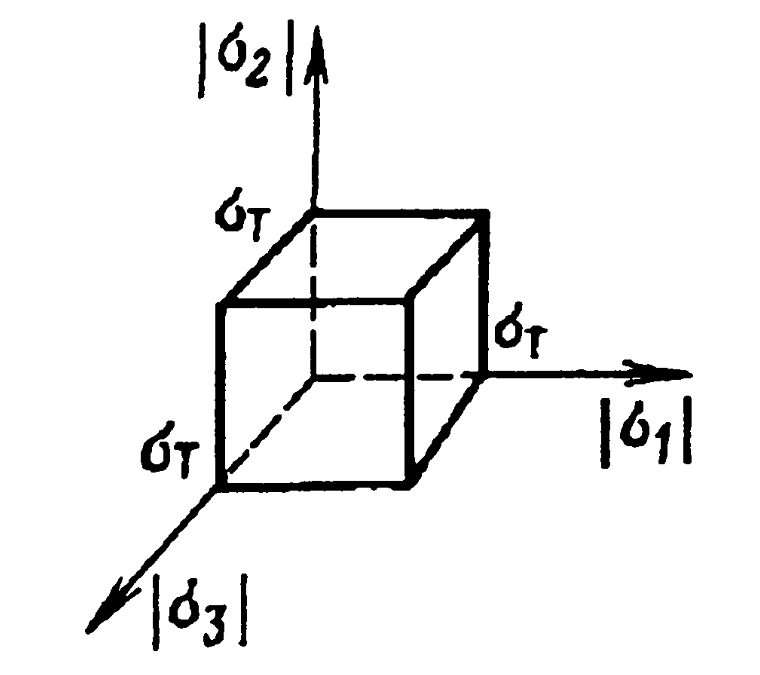
\includegraphics[width=0.3\textwidth]{png/destruction-criteria-one.png}}
\caption{Предельная поверхность для критерия нормальных напряжений.}
\end{figure}

Данный критерий удовлетворительно описывает разрушение хрупких материалов при напряженных состояниях, близким к одноосным. Явления пластического течения данный критерий описывает неудовлетворительно. Таким образом, области срабатывания данного критерия в хрупких материалах можно рассматривать как области потенциального разрушения отколом, а также области зарождения трещин \cite{griffith, orowan}.


\subsubsection{Критерий наибольших линейных деформаций}

При использовании данного критерия пластическое деформирование пластического материала или разрушение хрупкого материала наступает при достижении наибольшей по модулю линейной деформацией удлиннения предельного значения $\epsilon_*$. Предельная поверхность при этом имеет вид четырехгранной призмы в пространстве главных напряжений.

Данный критерий не получил большого распространения и имеет на практике достаточно нишевые области применения в тех задачах, которые так или иначе сводятся к плоскому деформированному состоянию \cite{selivanov}.


\subsubsection{Критерий Треска}

Критерий Треска основывается на наибольших касательных напряжениях. При использовании данного критерия пластическое деформирование пластического материала или разрушение хрупкого материала наступает при достижении наибольшим касательным напряжением предельного значения
\begin{equation}
\tau_{max} = \sigma_1 - \sigma_3 > \tau_*.
\end{equation}
Предельная поверхность для критерия Треска имеет в пространстве главных напряжений вид шестигранной призмы, равнонаклонённой к осям координат.

Критерий Треска удовлетворительно описывает пластическое деформирование металлов. Разрушения хрупких материалов данный критерий описывает не очень хорошо. Таким образом, области срабатывания данного критерия можно рассматривать как области потенциального разрушения для материалов, для которых свойственно пластическое разрушение сдвигом.


\begin{figure}[h]
\center{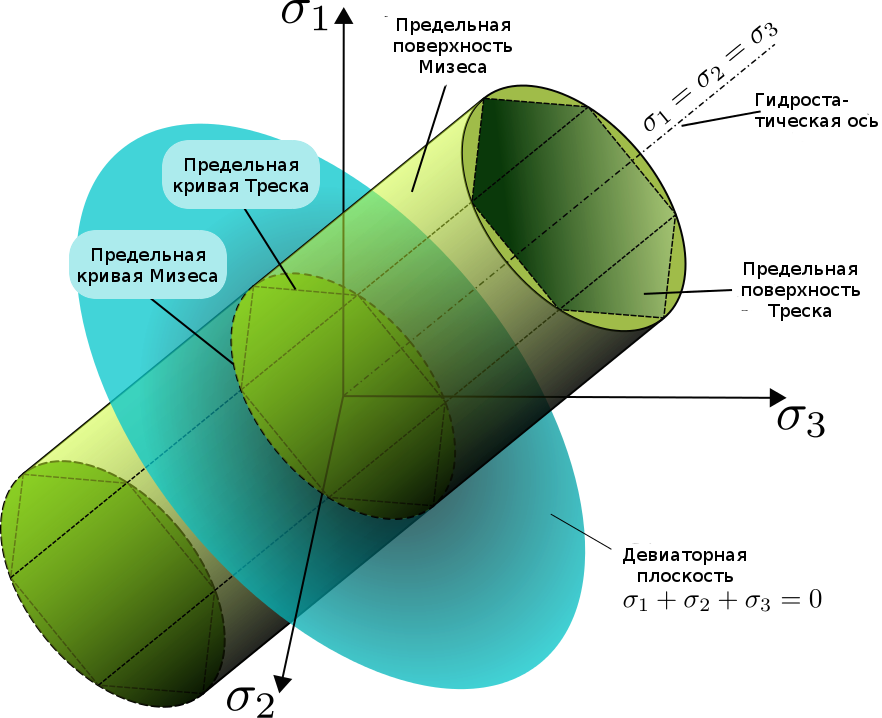
\includegraphics[width=0.5\textwidth]{png/yield_surfaces.png}}
\caption{Предельные поверхности для критерия Треска и критерия Мизеса.}
\end{figure}


\subsubsection{Критерий Мизеса}

Критерий Мизеса основывается на максимальной удельной энергии изменения формы. В случае линейной упругости полная удельная энергия деформированного тела представляется в виде суммы удельной энергии изменения объема и удельной энергии изменения формы. По определению критерия Мизеса пластическое деформирование пластического материала или разрушение хрупкого материала наступает при достижении удельной энергией изменения формы определенного значения.

Математически критерий Мизеса выражается через девиатор тензора напряжений:

\begin{equation}
\label{von_mises_criteria_generic}
J_2 \ge k^2,
\end{equation}
где $J_2$ - второй инвариант девиатора, а $k$ - предел текучести на сдвиг. Отсюда следует простая запись критерия Мизеса через компоненты тензора напряжений:
\begin{align}
\label{von_mises_criteria_components}
k^2 \le J_2 &= \frac{1}{2}s_{ij}s_{ji} = -s_1s_2 - s_2s_3 - s_3s_1 = \nonumber\\
 &= \frac{1}{6}[(\sigma_{xx} - \sigma_{yy})^2 + (\sigma_{yy} - \sigma_{zz})^2 + (\sigma_{xx} - \sigma_{zz})^2 ] + \sigma_{xy}^2 + \sigma_{yz}^2 + \sigma_{xz}^2.
\end{align}

Или через главные напряжения:
\begin{equation}
\label{von_mises_criteria_principal_stresses}
k^2 \le \frac{1}{6}[(\sigma_1 - \sigma_2)^2 + (\sigma_2 - \sigma_3)^2 + (\sigma_3 - \sigma_1)^2 ].
\end{equation}

Величина эквивалентного напряжения (напряжение Мизеса) в этом случае имеет вид:
\begin{equation}
\label{von_mises_equivalent_stress}
\sigma_e = \sqrt{ 3 J_2 } = \sqrt{ \frac{ (\sigma_1 - \sigma_2)^2 + (\sigma_2 - \sigma_3)^2 + (\sigma_3 - \sigma_1)^2 }{2} }.
\end{equation}

Предельная поверхность для критерия Мизеса имеет в пространстве главных напряжений вид цилиндра, равнонаклонённого к осям координат. Внутрь цилиндра вписана шестигранная призма, соответствующая критерию Треска. Максимальное различие критериев соответствует максимальному расстоянию между окружностью и вписанным в нее шестиугольником
\begin{equation}
\frac{\delta}{R} = \frac{R(1-cos(\pi/6))}{R} = 0.134.
\end{equation}
Таким образом, для решения технических задач критерии Мизеса и Треска можно считать эквивалентными. Принципиально, что критерии Мизеса и Треска зависят только от девиатора тензора напряжений, но не зависят от гидростатической части тензора.

Критерий Мизеса, так же как и критерий Треска, удовлетворительно описывает разрушение пластических материалов сдвигом и переход пластических материалов в состояние пластического течения. Из двух близких критериев - Мизеса и Треска - в дальнейшем используется критерий Мизеса, так как его удобнее реализовывать численно.


\subsubsection{Критерий Мора}

Критерий Мора сформулирован для материалов, обладающих разными пределами прочности при сжатии и при растяжении. Критерий учитывает как нормальные, так и касательные напряжения.

В основе критерия Мора лежит теория сухого трения Кулона. Критерий Мора основан на предположении, что разрушение возникает вследствие возникновения внутреннего скольжения в среде. Критерий предполагает, что скольжение возникает на площадках, проходящих через ось $\sigma_2$ в пространстве главных напряжений. Также предполагается, что напряжение $\sigma_2$ не влияет на возникновение скольжения, поэтому возникновение скольжения полностью описывается максимальным и минимальным главными напряжениями $\sigma_1$ и $\sigma_3$. При этом если внутреннее скольжение возникает на некоторой площадке, то на нее действуют предельные нормальное и касательное напряжения $\sigma_n$ и $\tau_n$, причем значение $\tau_n$ зависит от $\sigma_n$. Таким образом, в соответствии с критерием Мора, пластическое течение или хрупкое разрушение материала наступает тогда, когда касательное напряжение в плоскости скольжения увеличивается до определенного значения, зависящего от нормального напряжения в той же плоскости.

Математическая формулировка критерия Мора:
\begin{equation}
\label{mohr_criteria}
\tau_n = \sigma_n\tan(\phi) + c,
\end{equation}
где $\sigma_n$ - нормальное напряжение, $\tau_n$ - касательное напряжение, $\phi$ - угол внутреннего трения, $c$ - коэффициент когезии. Нетрудно заметить, что при $\phi = 0$ критерий Мора переходит в критерий Треска.

При этом
\begin{align}
\sigma &= \sigma_m - \tau_m \sin\phi, \nonumber\\
\tau &= \tau_m \cos\phi,
\end{align}

где
\begin{align}
\tau_m &= \frac{\sigma_1-\sigma_3}{2} \nonumber\\
\sigma_m &= \frac{\sigma_1+\sigma_3}{2} 
\end{align}.

Таким образом, критерий может быть альтернативно записан в форме:
\begin{equation}
\tau_m = \sigma_m \sin\phi + c \cos\phi.
\end{equation}

В трехмерном случае критерий имеет более сложный вид:
\begin{align}
  \pm\cfrac{\sigma_1 - \sigma_2}{2} & = \left[\cfrac{\sigma_1 + \sigma_2}{2}\right]\sin(\phi) + c\cos(\phi) \nonumber\\
  \pm\cfrac{\sigma_2 - \sigma_3}{2} & = \left[\cfrac{\sigma_2 + \sigma_3}{2}\right]\sin(\phi) + c\cos(\phi) \nonumber\\
  \pm\cfrac{\sigma_3 - \sigma_1}{2} & = \left[\cfrac{\sigma_3 + \sigma_1}{2}\right]\sin(\phi) + c\cos(\phi)
\end{align}.

Предельная поверхность в этом случае в пространстве главных напряжений имеет вид конуса, сечение которого девиаторными плоскостями представляют собой шестиугольники.

\begin{figure}[h]
\center{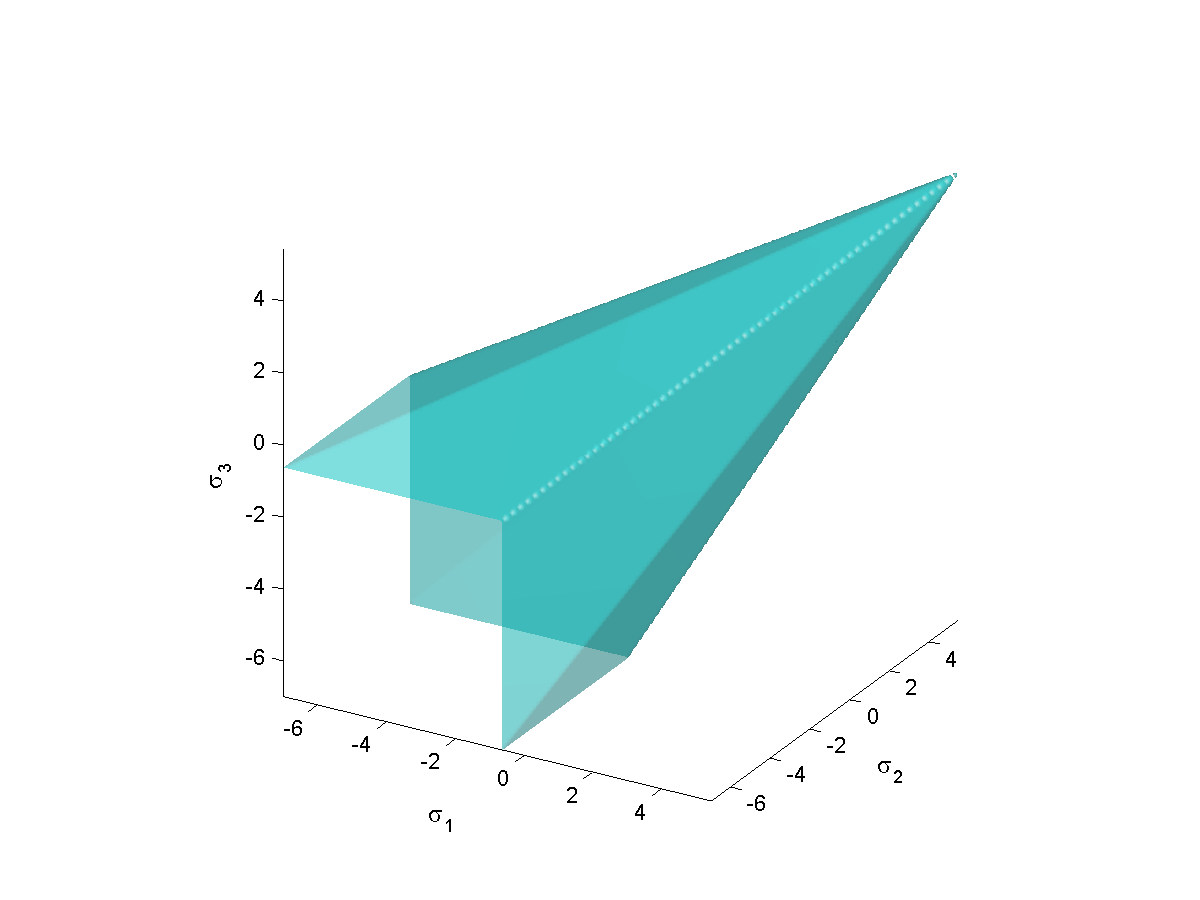
\includegraphics[width=0.5\textwidth]{png/mohr-criteria.png}}
\caption{Предельная поверхность для критерия Мора с параметрами $c = 2, \phi = -\pi/9$.}
\end{figure}

Математическая формулировка по-прежнему имеет вид \ref{mohr_criteria}, но $\tau_n$ и $\sigma_n$ теперь имеют смысл нормального и касательного напряжения к некоторой произвольной площадке в трехмерном пространстве.

Если рассматриваемая площадка задана нормалью
\begin{equation}
\mathbf{n} = n_1~\mathbf{e}_1 + n_2~\mathbf{e}_2 + n_3~\mathbf{e}_3,
\end{equation}
где $\mathbf{e}_i,~~ i=1,2,3$ - ортонормированный базис, то напряжение, действующее на площадку, имеет вид
\begin{equation}
\mathbf{t} = n_i~\sigma_{ij}~\mathbf{e}_j.
\end{equation}.

Величина напряжения очевидно
\begin{equation}
|\mathbf{t}| = \sqrt{ (n_j~\sigma_{1j})^2 + (n_k~\sigma_{2k})^2 + (n_l~\sigma_{3l})^2},
\end{equation}

а нормальная составляющая
\begin{equation}
\sigma = \mathbf{t}\cdot\mathbf{n} = n_i~\sigma_{ij}~n_j.
\end{equation}

В этом случае касательная составляющая выражается как
\begin{equation}
\tau = \sqrt{|\mathbf{t}|^2 - \sigma^2}
\end{equation}

В покомпонентной записи получаем:
\begin{align}
\sigma &= n_1^2 \sigma_{11} + n_2^2 \sigma_{22} + n_3^2 \sigma_{33} + 
	2(n_1 n_2 \sigma_{12} + n_2 n_3 \sigma_{23} + n_3 n_1 \sigma_{31}), \nonumber\\
\tau &= ((n_1\sigma_{11} + n_2\sigma_{12} + n_3\sigma_{31})^2 +
	(n_1\sigma_{12} + n_2\sigma_{22} + n_3\sigma_{23})^2 + \nonumber\\
 &	+ (n_1\sigma_{31} + n_2\sigma_{23} + n_3\sigma_{33})^2 - \sigma^2)^{1/2}
\end{align}

Если базисные векторы $\mathbf{e}_i,~~ i=1,2,3$ сонаправлены с главными напряжениями $\sigma_1, \sigma_2, \sigma_3$, то получаем окончательное выражение в виде
\begin{align}
    \sigma &= n_1^2 \sigma_{1} + n_2^2 \sigma_{2} + n_3^2 \sigma_{3}, \nonumber\\
    \tau &= \sqrt{(n_1\sigma_{1})^2 + (n_2\sigma_{2})^2 + (n_3\sigma_{3})^2 - \sigma^2} = \nonumber\\
         &= \sqrt{n_1^2 n_2^2 (\sigma_1-\sigma_2)^2 + n_2^2 n_3^2 (\sigma_2-\sigma_3)^2 + 
                 n_3^2 n_1^2 (\sigma_3 - \sigma_1)^2}
\end{align}.


\subsubsection{Критерий Друкера-Прагера}

Критерий Друкера-Прагера задается следующей формулой:
\begin{equation}
\sqrt{J_2} = A + B~I_1,
\end{equation}
где $I_1$ — первый инвариант тензора напряжений, а $J_2$ — второй инвариант девиатора тензора напряжений. Константы $A, B$ определяются экспериментально.

С эквивалентным напряжением Мизеса и с гидростатической частью тензора критерий Друкера-Прагера связан следующим соотношением
\begin{equation}
\sigma_e = a + b~p,
\end{equation}
где $\sigma_e$ — эквивалентное напряжение Мизеса, $p$ — гидростатическое напряжение, $a,b$ - константы материала.

Через главные напряжения критерий может быть выражен следующим образом:
\begin{equation}
\sqrt{\cfrac{1}{6}\left[(\sigma_1-\sigma_2)^2+(\sigma_2-\sigma_3)^2+(\sigma_3-\sigma_1)^2\right]} = A + B~(\sigma_1+\sigma_2+\sigma_3).
\end{equation}

При этом для случая одноосного растяжения получаем:
\begin{equation}
\cfrac{1}{\sqrt{3}}~\sigma_t = A + B~\sigma_t ~,
\end{equation}
а для одноосного сжатия:
\begin{equation}
\cfrac{1}{\sqrt{3}}~\sigma_c = A - B~\sigma_c ~.
\end{equation}

Из этих уравнений следует связь параметров $A, B$ с пределами прочности при одноосном сжатии и одноосном растяжении:
\begin{align}
A = \cfrac{2}{\sqrt{3}}~\left(\cfrac{\sigma_c~\sigma_t}{\sigma_c+\sigma_t}\right), \nonumber\\
B = \cfrac{1}{\sqrt{3}}~\left(\cfrac{\sigma_t-\sigma_c}{\sigma_c+\sigma_t}\right).
\end{align}

Предельная поверхность Друкера-Прагера представляет собой сглаженный вариант предельной поверхности Мора.

\begin{figure}[h]
\center{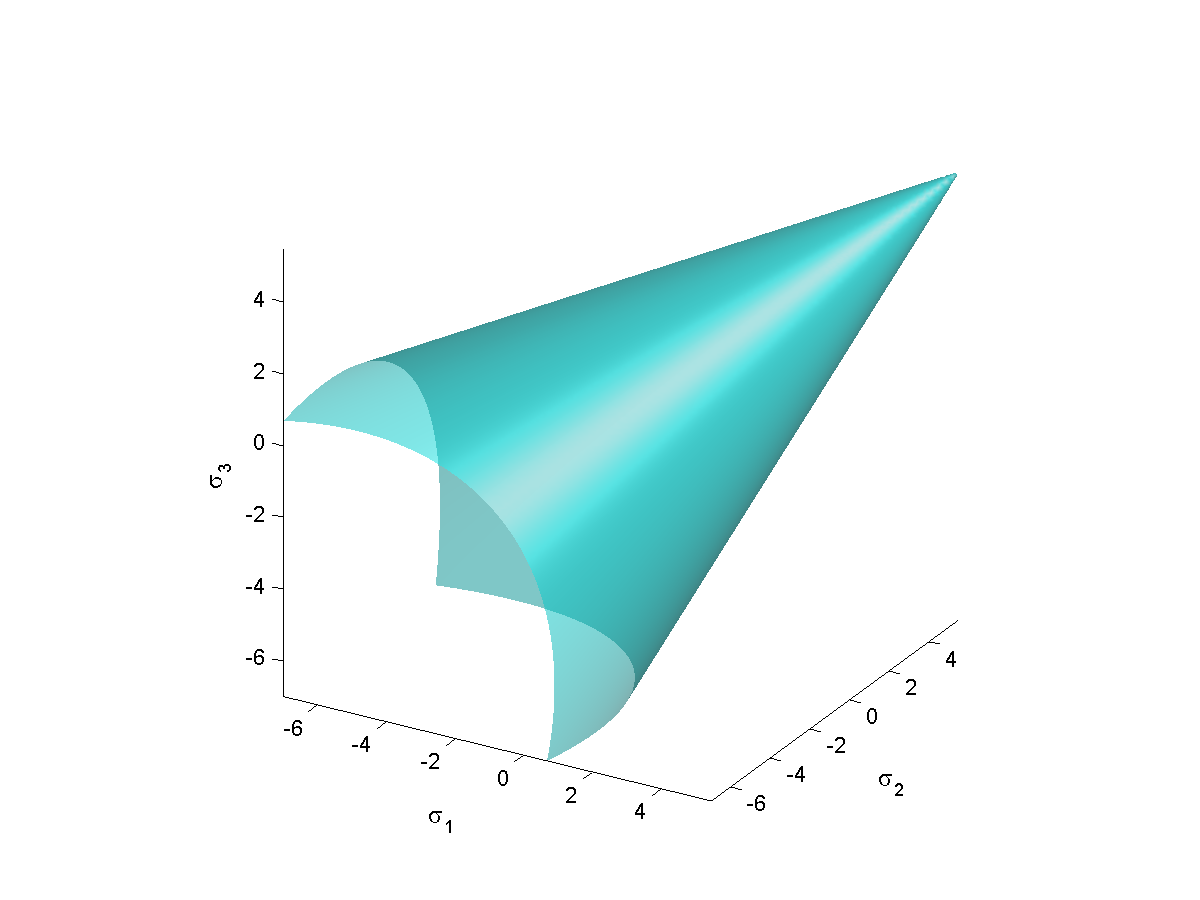
\includegraphics[width=0.5\textwidth]{png/druker-prager-criteria.png}}
\caption{Предельная поверхность для критерия Друкера-Прагера с параметрами $c = 2, \phi = -\pi/9$.}
\end{figure}

Если поверхность Друкера-Прагера описывает поверхность Мора, то связь коэффициентов $A, B$ с коэффициентом когезии и углом внутреннего трения имеет вид
\begin{align}
A = \cfrac{6~c~\cos\phi}{\sqrt{3}(3+\sin\phi)}, \nonumber\\
B = \cfrac{2~\sin\phi}{\sqrt{3}(3+\sin\phi)}.
\end{align}

Если поверхность Друкера-Прагера вписана в поверхность Мора, то уравнения принимают вид
\begin{align}
A = \cfrac{6~c~\cos\phi}{\sqrt{3}(3-\sin\phi)}, \nonumber\\
B = \cfrac{2~\sin\phi}{\sqrt{3}(3-\sin\phi)}.
\end{align}

В более сложных случаях критерий может иметь второй порядок относительно инварианта $I_1$ и, соответственно, гидростатической части тензора:
\begin{equation}
J_2 = (A + B~I_1)^2 = a + b~I_1 + c~I_1^2
\end{equation}

\subsubsection{Адгезионная прочность}

Отдельное место среди критериев разрушения занимает адгезионная прочность. Если все рассмотренные ранее критерии описывают разрушение изотропного материала, то адгезионная прочность относится к разрушению контакта между телами (или областями одного тела). Адгезионная прочность описывает такие явления как разделение слоев композита или выдергивание волокон из матрицы композита.

Критерий разрушения контакта строится аналогично рассмотренным критериям наибольших нормальных и касательных напряжений. Только рассматриваются теперь напряжения не в объеме материала, а на контактной границе границе.


